\documentclass{beamer}
\usepackage{listings}
\usetheme{Copenhagen}
\usecolortheme{beaver}
\setbeamertemplate{navigation symbols}{}
\setbeamertemplate{footline}{\parbox[t][12pt][c]{12pt}{~\scriptsize\insertframenumber}}
% \usepackage{beamerthemesplit} // Activate for custom appearance

%%%%%%%%%%%%
% MVS: Language definitions
%
\renewcommand{\ttdefault}{pcr}
\lstset{
  basicstyle=\small\ttfamily,
  breaklines=true
}
\lstdefinelanguage{cvl}{
  morekeywords={generalize,to, with, other, at, zoom, levels, weigh, by, subject, and, create, constraint, as, not, exists, resolve, if, delete, select, from, where, in, order, over, setup, teardown,force,min,level,for,allornothing,join,on,setup,group,having,index,temporary,table,drop,partition,merge,partitions},
  sensitive=false,
  morecomment=[l]{//},
  morecomment=[s]{/*}{*/},
  morestring=[b]",
}
\lstset{
  language=cvl
}


\title{Declarative Cartography}
\subtitle{In-Database Map Generalization of Spatial Datasets}
\author{\underline{Pimin Konstantin Kefaloukos}, Marcos Vaz Salles, \\Martin Zachariasen\\ \small{\emph{Computer Science Department (DIKU)}, \textbf{University of Copenhagen}}}

\date{\today}

\begin{document}

\frame{\titlepage}

\frame
{
  \frametitle{Motivation}
  \begin{itemize}
  \item \textbf{Imagine}: you're a \emph{journalist} and want to tell a story about restaurants in Z\"{u}rich \emph{using a map}.
  \item \textbf{Database}: You have a \emph{database} of restaurants (unique ID, location, star rating, name etc.)
  \item Simply showing all the records creates a mess (see picture)
  \item Generalization of thematic data is an important problem, with increasing use cases in \emph{social networks}, \emph{data journalism} etc
  \end{itemize}
  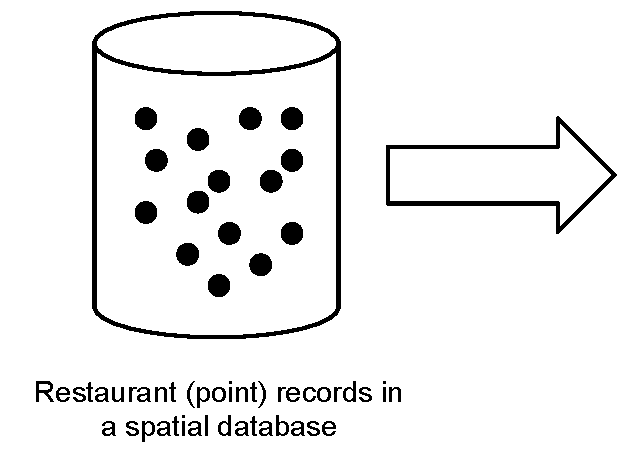
\includegraphics[scale=0.5]{figs/spatial-database-with-points.pdf} 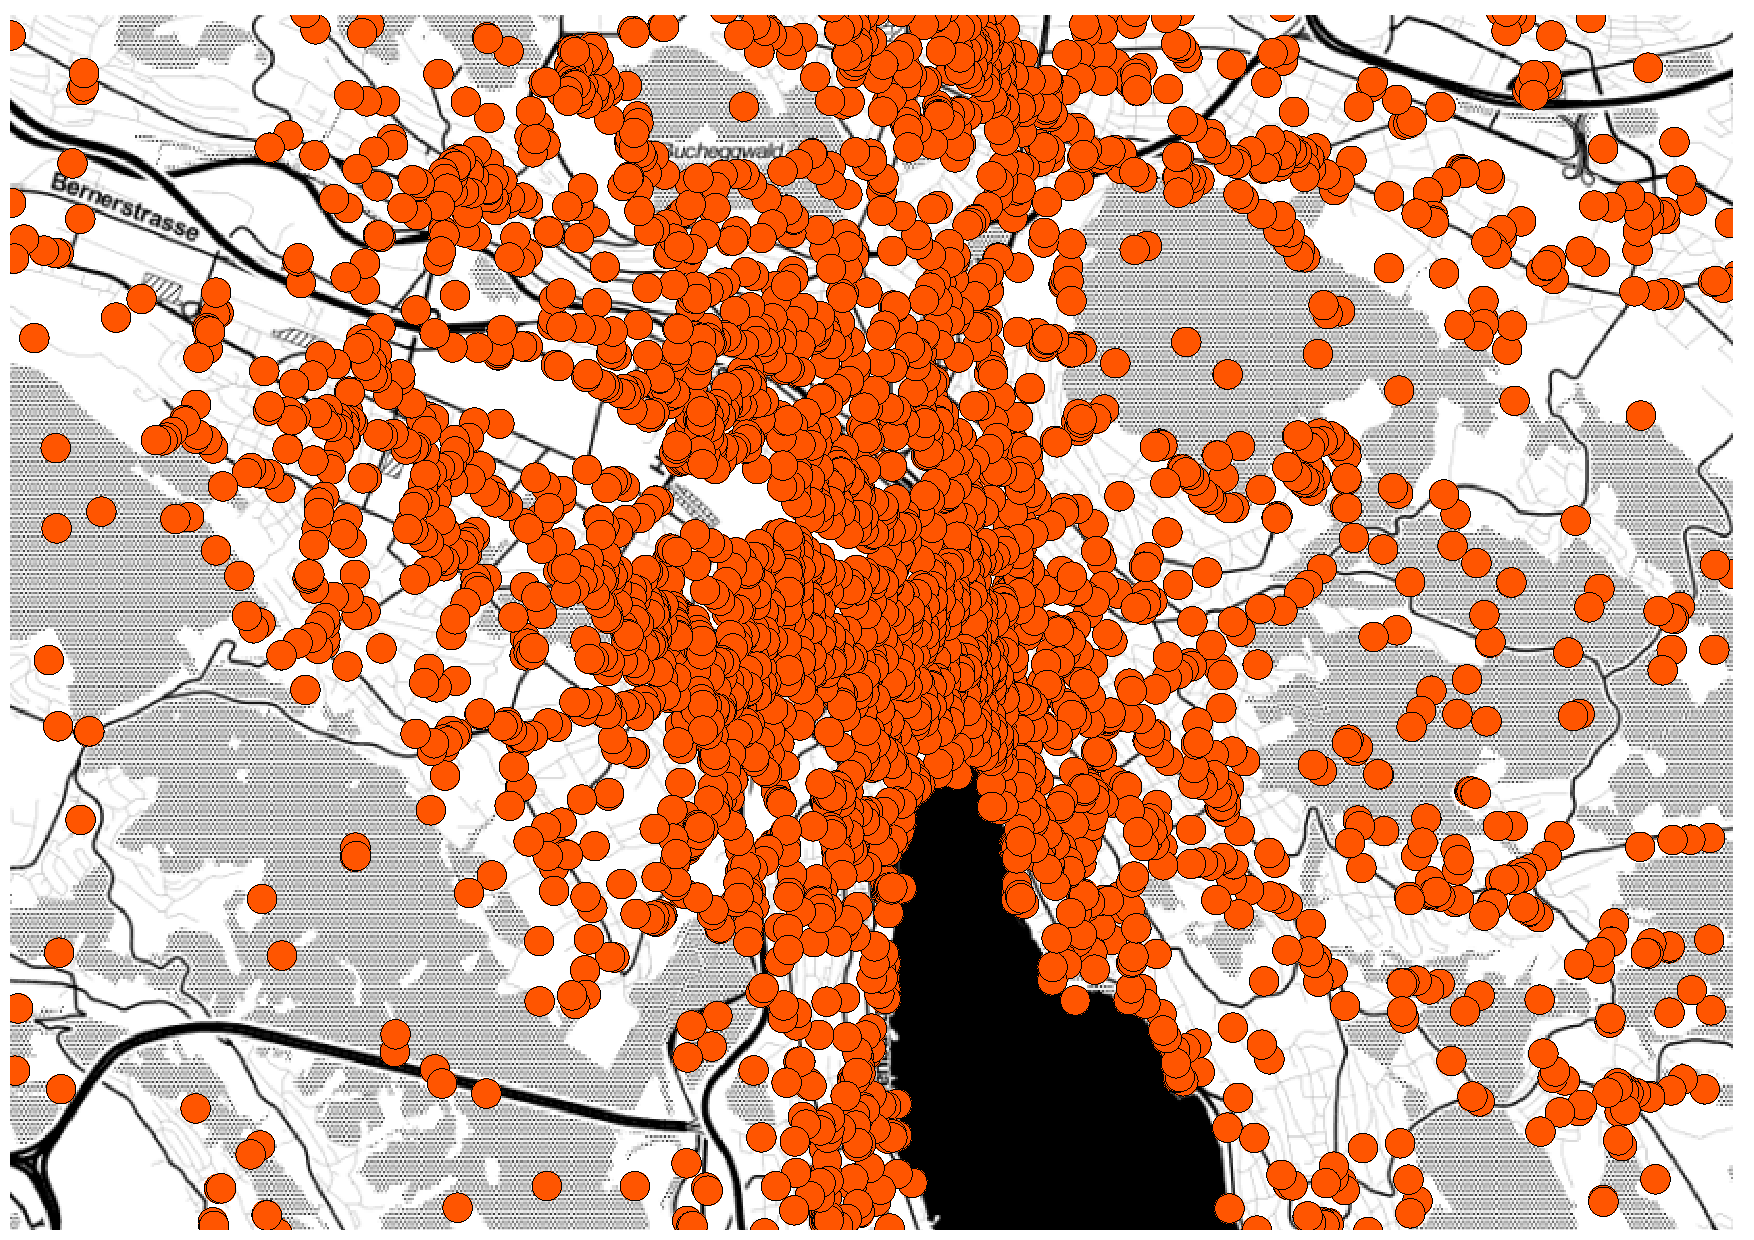
\includegraphics[scale=0.18]{figs/zurich-unfiltered.pdf}
}

% Setting stage
\frame[t]
{
  \frametitle{What a good (thematic) map might look like}
\begin{columns}[t]
	\begin{column}[l]{6cm}
		\begin{itemize}[<+->]
			\item Records should appear \emph{gradually} when zooming in, i.e. \emph{constant information~density}
			\item ``Important'' records should get priority
			\item Visible records should \emph{remain visible} when zooming in
			\item There should be some way of controlling \emph{layout}
		\end{itemize}
	\end{column}
	\begin{column}[l]{6cm}
    \begin{figure}
    	\includegraphics<1>[scale=0.18]{figs/zoom12.pdf}
        \includegraphics<2>[scale=0.18]{figs/zoom13.pdf}
        \includegraphics<3>[scale=0.18]{figs/zoom14.pdf}
        \includegraphics<4>[scale=0.18]{figs/zoom15.pdf}
    \end{figure}                            
\end{column}
\end{columns}
}

% Setting stage
\frame[t]
{
  \frametitle{Spatial databases}
	\begin{itemize}[<+->]
		\item Spatial data is often stored in a \emph{spatial database}
		\item They have powerful capabilities
		\item \emph{joins}, \emph{sorting}, \emph{spatial indexing} and \emph{spatial functions}
	\end{itemize}
	\begin{center}
	\begin{figure}
    		\includegraphics<1>[scale=0.3]{figs/cvl-powerful-database.pdf}
    		\includegraphics<2>[scale=0.3]{figs/cvl-powerful-database.pdf}
		\includegraphics<3>[scale=0.3]{figs/cvl-powerful-database-2.pdf}
	\end{figure}       
	\end{center}                     
}

\frame[t]
{
  \frametitle{Situation}
	\begin{itemize}[<+->]
		\item Normally data is pulled out of the \emph{database} for processing tasks like generalization
		\item Generalization algorithms are usually implemented in external software
		\item After the processing is done the data is put back into the database
		\item \emph{Several drawbacks}: re-inventing the wheel, memory and bandwidth limits, development and deployment costs, 
	\end{itemize}
	\begin{center}
	\begin{figure}
    		\includegraphics<1>[scale=0.3]{figs/cvl-external-software-out.pdf}
    		\includegraphics<2>[scale=0.3]{figs/cvl-external-software-proc.pdf}
		\includegraphics<3>[scale=0.3]{figs/cvl-external-software-in.pdf}
		\includegraphics<4>[scale=0.3]{figs/cvl-external-software-rest.pdf}
	\end{figure}       
	\end{center}                     
}

\frame[t]
{
  \frametitle{Why not use the database itself?}
	\begin{itemize}[<+->]
		\item Instead, we state generalization in terms of a high-level language
		\item The language is translated to a low-level database program
		\item We move code-to-data instead of moving data-to-code

	\end{itemize}
	\begin{center}
	\begin{figure}
    		\includegraphics<1>[scale=0.3]{figs/cvl-state-intension.pdf}
    		\includegraphics<2>[scale=0.3]{figs/cvl-compile-statement.pdf}
		\includegraphics<3>[scale=0.3]{figs/cvl-code-to-data.pdf}
	\end{figure}       
	\end{center}                     
}


\frame[t]
{
  \frametitle{In-database processing}
	\begin{itemize}
		\item The low-level program can of course exploit capabilities of spatial databases, such as indexing and spatial functions
	\end{itemize}
	\begin{center}
	\begin{figure}
    		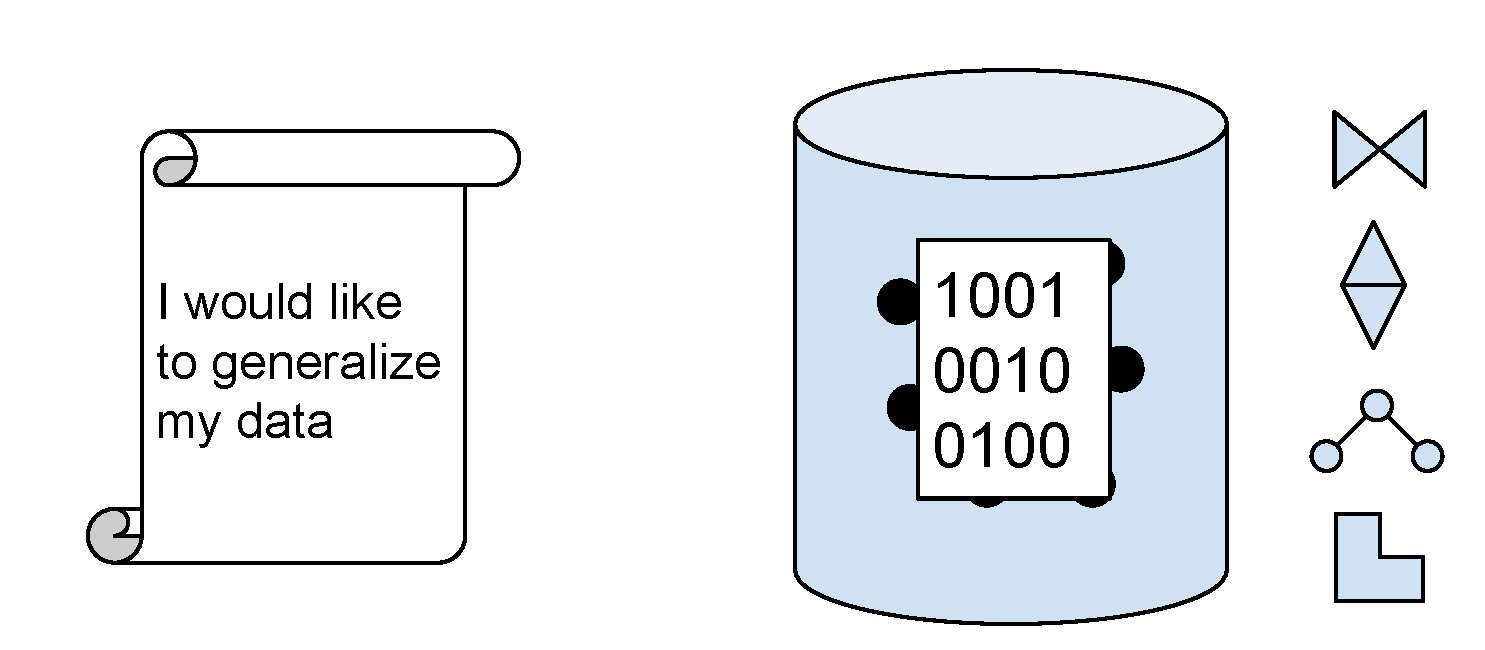
\includegraphics[scale=0.4]{figs/cvl-code-to-data-exploit.pdf}
	\end{figure}       
	\end{center}                     
}

\frame[t]
{
  \frametitle{The language}
	\begin{itemize}[<+->]
		\item High-level language has a \texttt{GENERALIZE} statement and a \texttt{CREATE CONSTRAINT} statement
		\item The \texttt{GENERALIZE} statement produces a generalized database table from a table of base data
		\item The \texttt{CREATE CONSTRAINT} statement is used to define new spatial constraints, e.g. proximity
		\item The table produced by \texttt{GENERALIZE} has a \texttt{min\_zoom} column added to all records
	\end{itemize}
	\begin{center}
  		\fbox{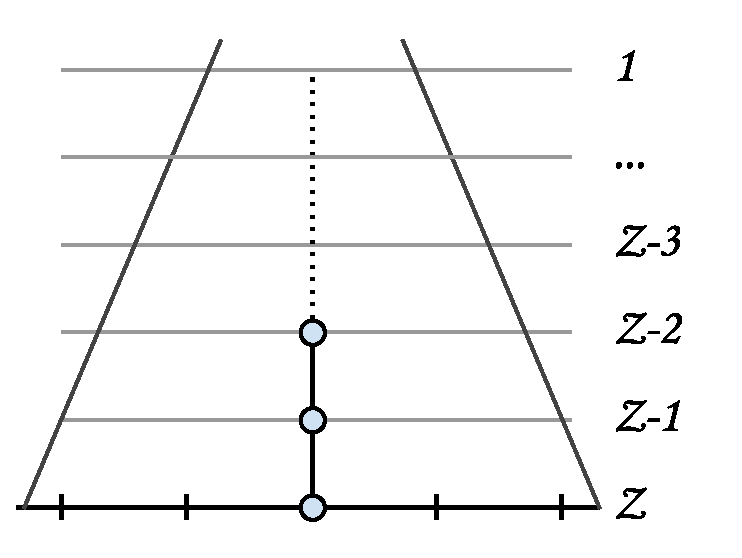
\includegraphics[scale=0.30]{figs/cvl-problem.pdf}}
  	\end{center}
}

% Introduce syntax
\begin{frame}[fragile,t]
  \frametitle{Language example}
  \begin{description}[<+->]
  \item
  \begin{lstlisting}
GENERALIZE restaurants 
\end{lstlisting}
  \item
\begin{lstlisting}
TO restaurants2
\end{lstlisting}
  \item
\begin{lstlisting}
AT 20 ZOOM LEVELS
\end{lstlisting}
  \item
\begin{lstlisting}
WEIGH BY star_rating
\end{lstlisting}
  \item
\begin{lstlisting}    
SUBJECT TO proximity 10 AND density 64
\end{lstlisting}    
  \end{description}
\end{frame}

% Introduce syntax
\begin{frame}[fragile,t]
  \frametitle{Language example}
  \begin{itemize}
  \item Result of generalization viewed at zoom-level 16
  \end{itemize}
  \begin{center}
  	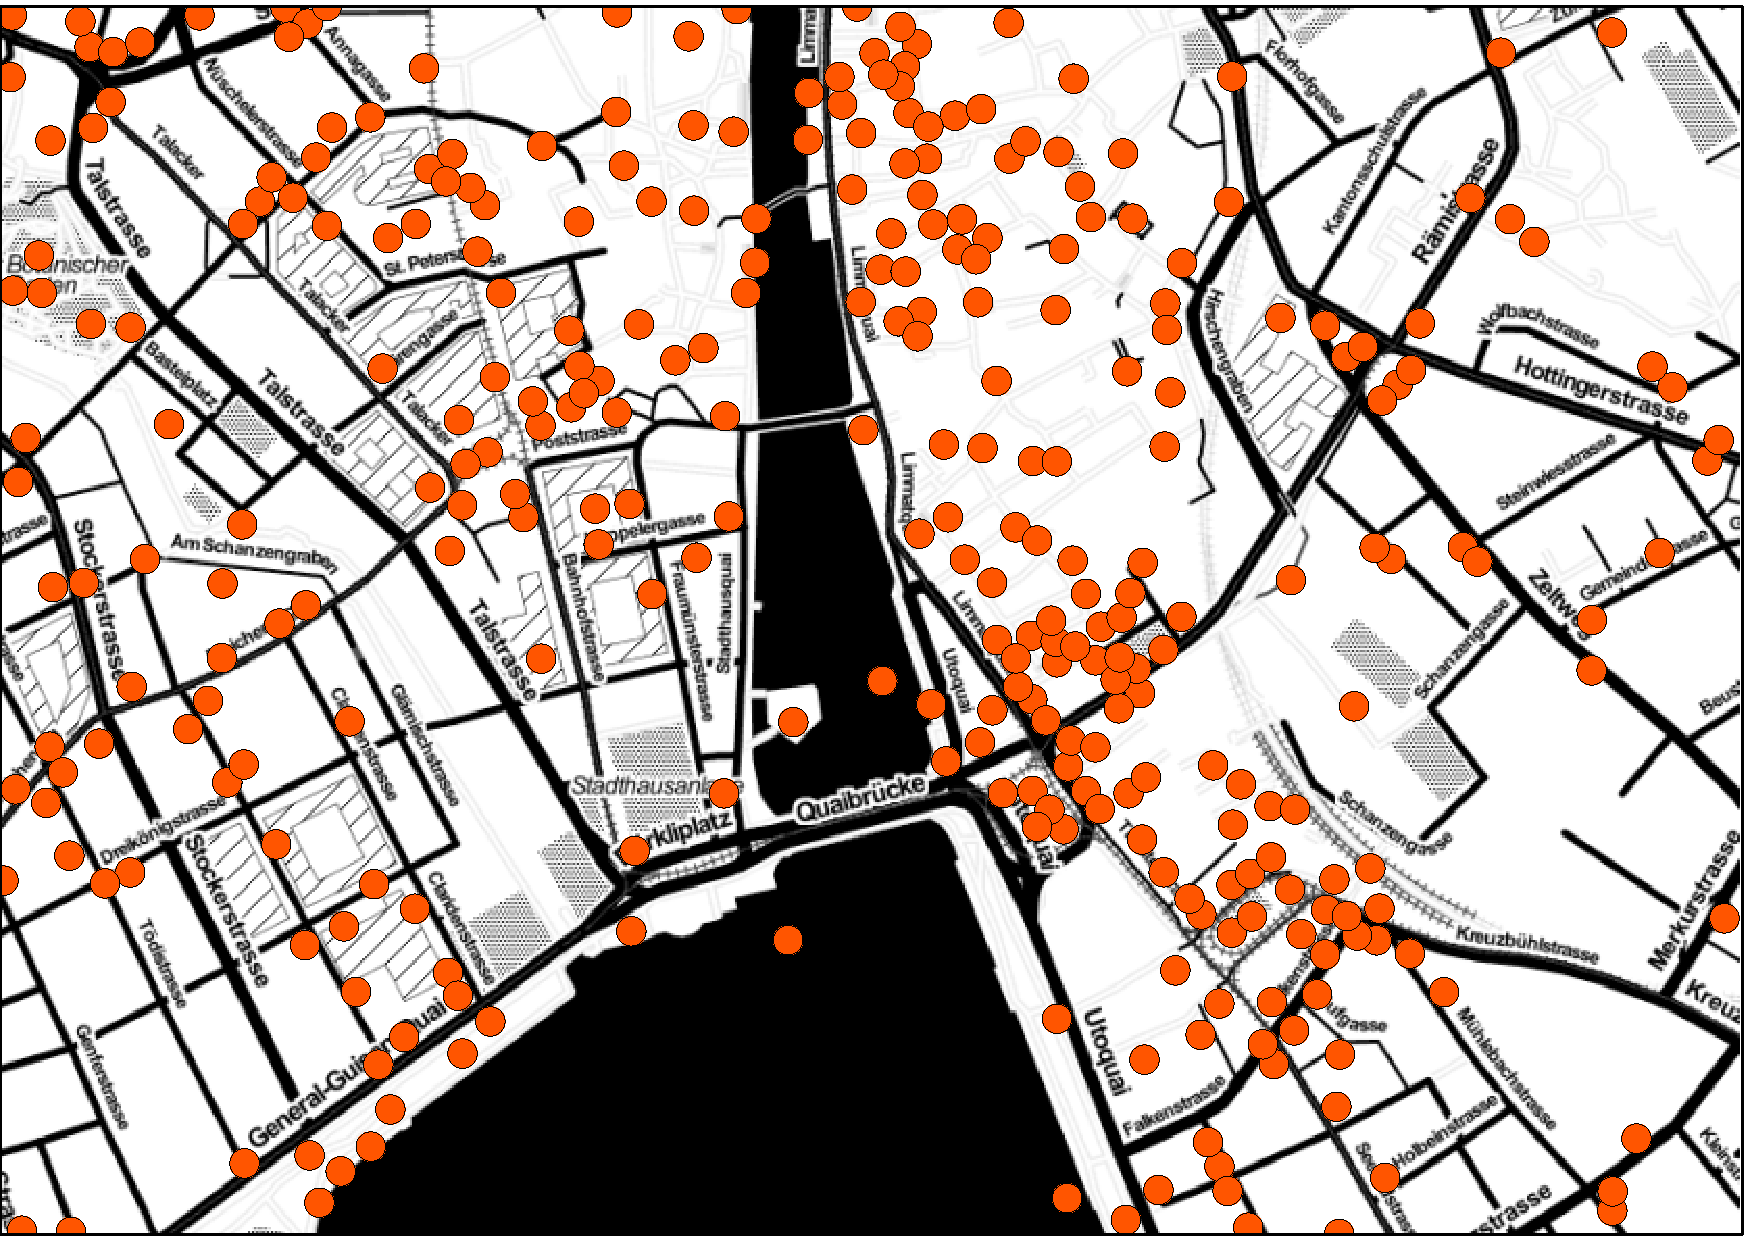
\includegraphics[scale=0.30]{figs/zoom16.pdf}
  \end{center}

\end{frame}


\frame[t]
{
  \frametitle{Computing solutions}
	\begin{itemize}[<+->]
	\item Combination of record weights and spatial constraints (proximity, density) present a natural optimization problem
	\item Represent generalization problem as instances of set multicover problem (SMP)
	\item Reuse existing algorithms for SMP (database implementations)
	\item Solution to SMP $\rightarrow$ records that should be filtered out at given zoom level
	\end{itemize}
	\begin{center}
  		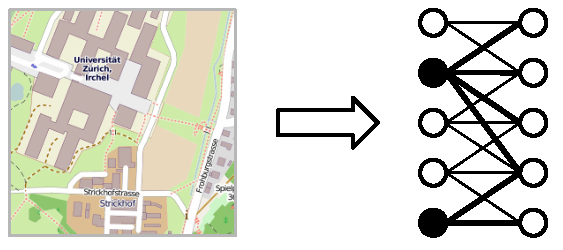
\includegraphics[scale=0.70]{figs/cvl-spatial-to-nonspatial.pdf}
  	\end{center}
}

\frame[t]
{
  \frametitle{Computing solutions}
	\begin{itemize}[<+->]
	\item Use auto-generated SQL queries to find records that violate constraints (conflict sets)
	\item For each conflict set filter out some number of records to resolve conflict
	\item Minimize combined weight of records that are filtered out over all zoom levels
	\end{itemize}
	
	\begin{center}
	\begin{figure}
  		\fbox{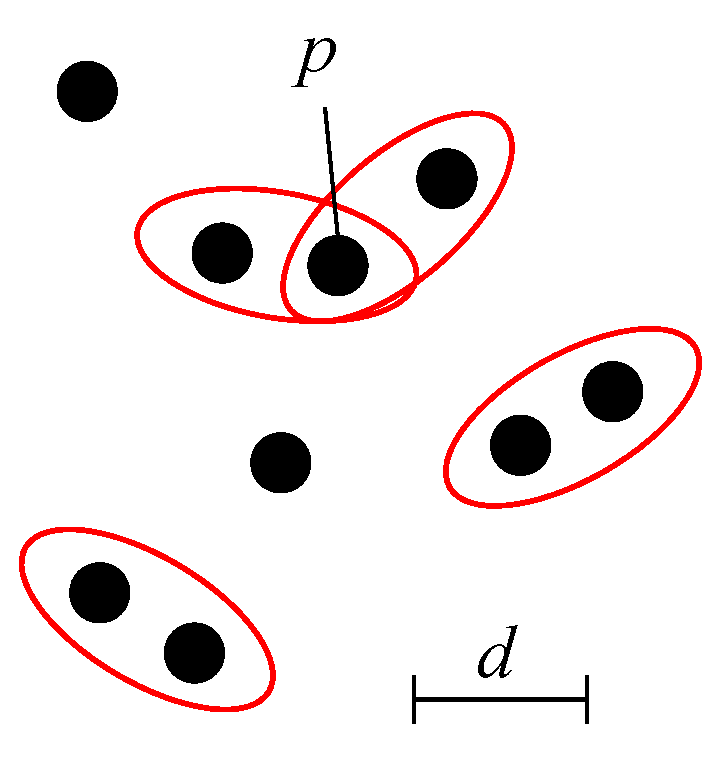
\includegraphics[scale=0.25]{figs/cvl-proximity-conflicts.pdf}}
	\caption{Four conflict sets generated by a proximity constraint}
	\end{figure}
  	\end{center}
}


\frame[t]
{
  \frametitle{Summary}
	\begin{itemize}
	\item Designed a high-level language for generalization called CVL
	\item Compiled to low-level database program and moved code-to-data
	\item Exploited correspondence to well-known optimization problem
	\item Also, method works with both points, lines and polygons
	\end{itemize}
	\begin{center}
	\begin{figure}
  		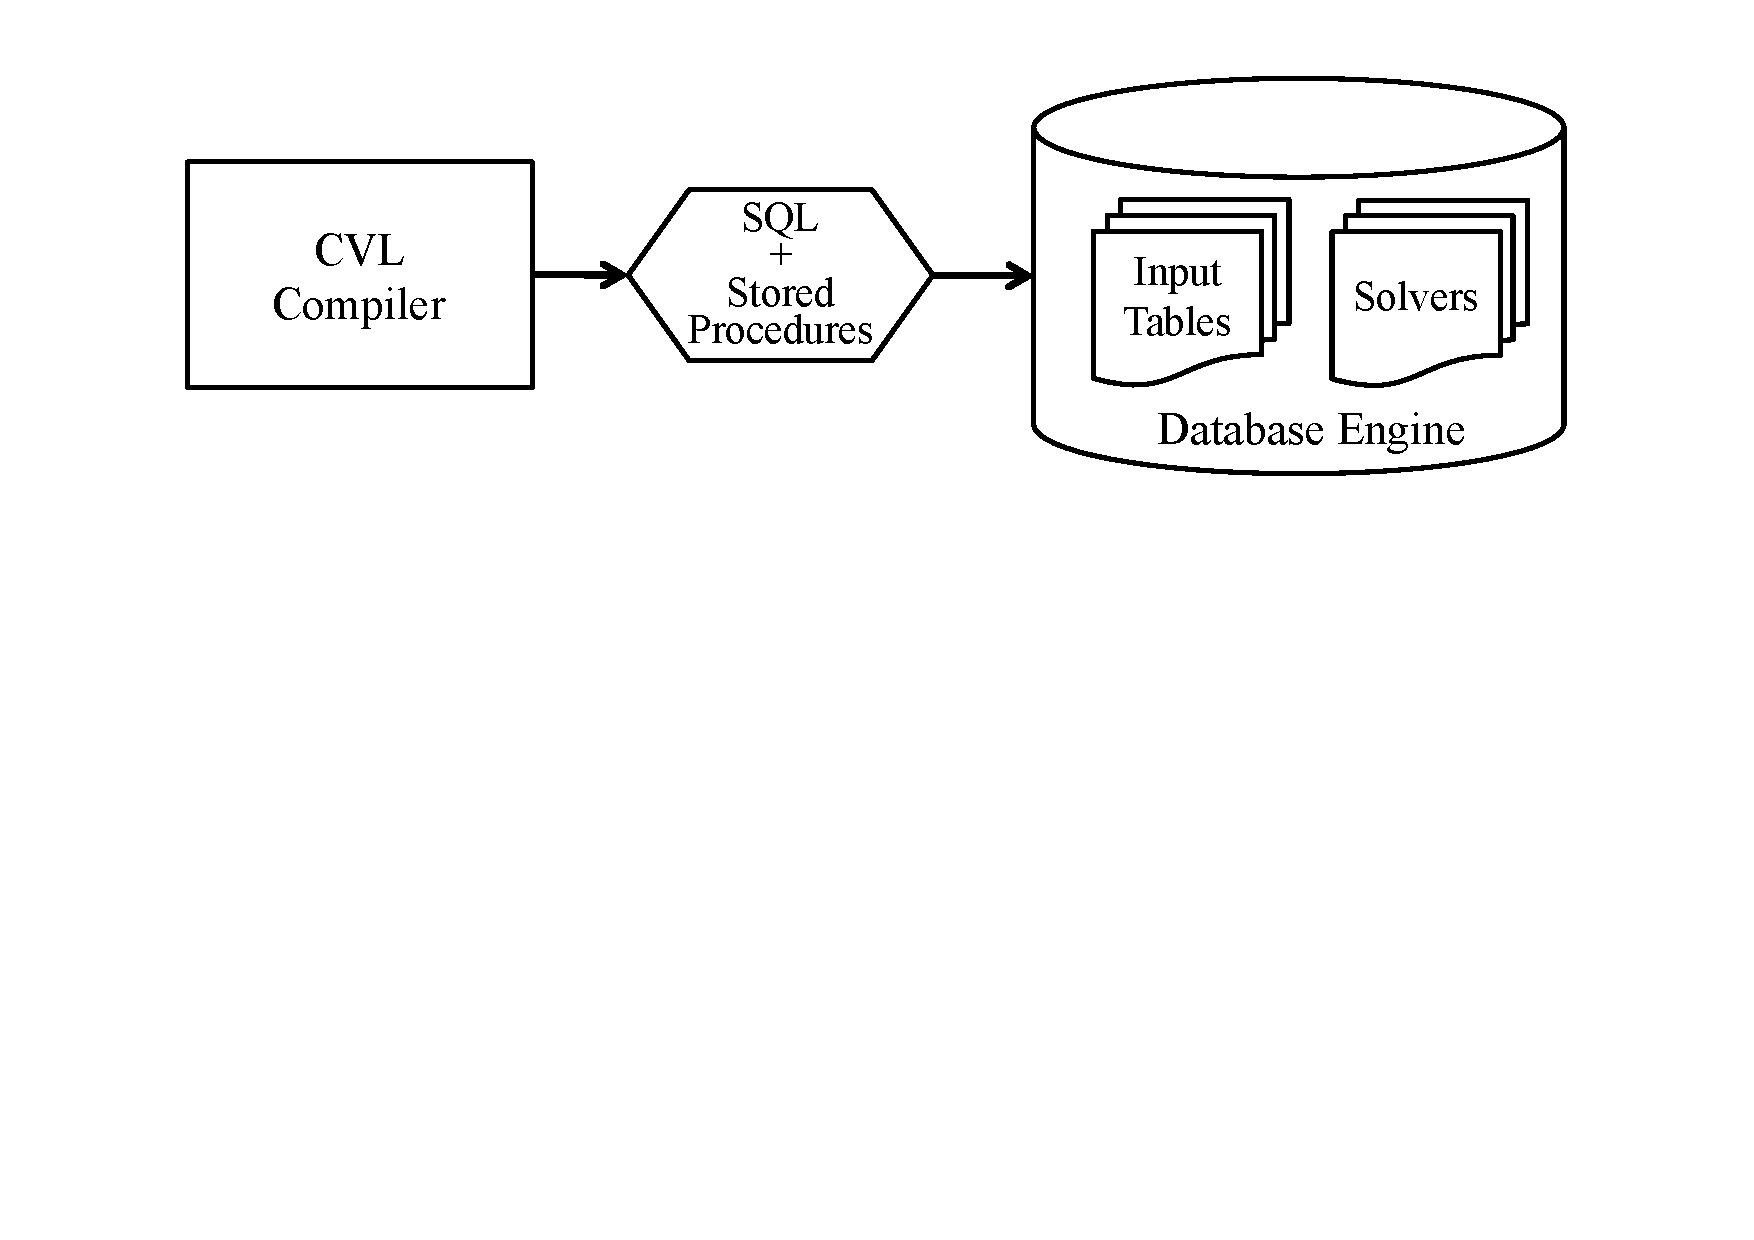
\includegraphics[scale=0.25]{figs/indatabase-execution.pdf}
	\caption{Architecture of CVL}
	\end{figure}
  	\end{center}
}

\frame[t]
{
  \frametitle{Future work}
	\begin{itemize}
	\item Implement aggregation as conflict resolution method
	\item Reduce dependencies of database program code
	\item Optimize low-level code generation
	\item Validate method in comprehensive user tests
	\item Identify areas where method can be further developed
	\end{itemize}
	\begin{center}
	\begin{figure}
  		\fbox{Thank you!}
	\end{figure}
	\end{center}
	\begin{center}
	  	Work will appear at ICDE '14 in Chicago, IL
	\end{center}	
}


\end{document}